
\tb{AT this point include the DEATH rate not useful}




As mentioned above, $\tau_p(\textbf{x},t)$ is part of the relaxation time of $\textbf{R}(\textbf{x},t)$. 
In addition, $\tau_p = a_p$ in most of the cases presented above. 
Consequently, according to the values measured in \ref{fig:tau_p} the microstructure relaxation time of dilute suspensions will be larger.

This implies that the terms on the left-hands side of \ref{eq:dt_R} may not be neglected and that direct closure for the microstructure in terms of $\phi$, $Ga$ and $\lambda$ may not be achievable at these large $\tau_p$. 

especially at $Ga = 50$, and may need a consequent amount of time to reach a steady state regime. 
In turns, this relaxation time will be reflected on the drift velocity between both phases, which is microstructure dependent. 
\begin{figure}
    \centering
    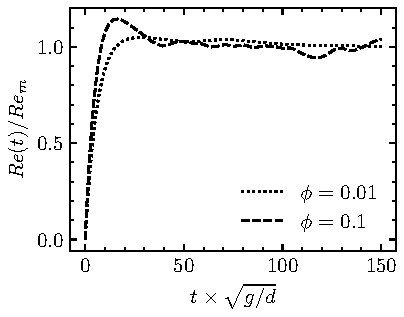
\includegraphics[height=0.325\textwidth]{image/HOMOGENEOUS_NEW/CA/Relax2.pdf}
    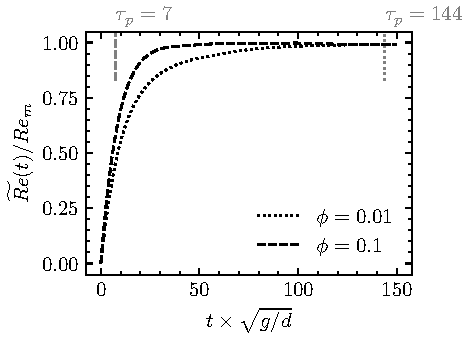
\includegraphics[height=0.35\textwidth]{image/HOMOGENEOUS_NEW/CA/Relax.pdf}
    \caption{
        (left) Average of the Reynolds number based on the instantaneous volume averaged drift velocity, $Re(t) = \rho_fU d /\mu_f$, with $U(t) = |\textbf{u}_p - \textbf{u}_f|$, divided by the mean Reynolds number $Re_m$ in terms of the dimensionless time. 
        (right) Running average of the Reynolds number $\widetilde{Re}(t)$ divided by the mean Reynolds number.
        For $\lambda = 1$ and $Ga = 50$ and two volumes fraction. 
        $\textbf{u}_p$ and $\textbf{u}_f$ are the particle and fluid phase volume averaged velocity at time $t$.
        The verticals gray lines indicate the values of $\tau_p$ all cases. 
        }
        \label{fig:relax}
\end{figure}
Indeed, in \ref{fig:relax} (right) we display the running average of the Reynolds number, based on the drift velocity, divided by the mean Reynolds number of the simulation for two values of $\phi = 0.01,0.1$ at $Ga = 50$ and $\lambda =1$. 
% It is seen that time, at which the simulation reaches a steady state regime is correlated with $\tau_p$. 
In this case we assume that two timescales are involved to bring the drift velocity to its statistically steady state regime. 
The first one is the particles' timescale, which is the time taken for a single particle to reach its own terminal velocity. 
The second timescale is the time taken for the microstructure to go from random, to its steady state microstructure. 
As a matter of fact, on \ref{fig:relax} we see that in the dilute regime ($\phi=0.01$) the rising velocity reaches its averaged value, at a time roughly equal to $100\sqrt{g/d}$ which is of the same order of magnitude than $\tau_p = 144\sqrt{g/d}$. 
On the contrary, when $\phi =0.1$ the averaged Reynolds number is indeed reached earlier ($t = 30\sqrt{g/d}$), despite the higher velocity fluctuations present in this case, see \ref{fig:relax} (left). 
The particle timescale is the same for both cases displayed \ref{fig:relax}, since only the volume fraction changes.
Additionally, the Statistical samples are supposed to be equivalent at same time since each  case posses the same number of droplets per domain. 
Thus, the changes in relaxation time is solely due to the microstructure relaxation timescale. 
Therefore, in support of the theory, $\tau_p$ seems capable of predicting the relaxation time of the microstructure.
The rising velocity of particles is directly correlated to the interphase drag force in sedimentation problems \citep{jackson1997locally}. 
Therefore, in the objective of finding closure terms for the averaged models, one must perform DNS for a time longer than $\tau_p$ plus the particle timescale, to allow the microstructure to relax adequately.
Then by performing an ensemble average procedure, one is able to build drag force models. 
Once established, these models will remain valid only under the condition where the timescale of the macroscopic flow significantly exceeds $\tau_p(\textbf{x},t)$ plus the particle timescale.
Indeed, these models have been built for relaxed microstructure and can be utilized only in this context.
Consequently, $\tau_p$ among other factors such as the particle relaxation time, provides a threshold value for the timescale not achievable in Euler-Euler models. 
